\newpage
\section*{6\quad Normalisation, and why depth is hard}
\addcontentsline{toc}{section}{6 Normalisation, and why depth is hard}
\startchapter{6}

\begin{chaptermap}
\emph{The problem:} real models stack dozens of blocks, and every block adds to the residual stream. What
happens to the size of the arrows after 48 additions? \emph{The steps:} measure it on untrained blocks (\S6.1);
fix it by resizing every arrow before it is used, with RMSNorm or LayerNorm, and see what each does to an arrow
geometrically (\S6.2); put the norm into our toy block and check its predictions (\S6.3); decide whether the
norm goes before or after each layer, with measurements (\S6.4). \emph{Where it ends:} with the block modern
models use, \emph{pre-norm}, and a measured reason for choosing it.
\end{chaptermap}

\machine{6}{You are here: Chapter 6 adds the \emph{norm} boxes. One sits in front of attention, one in front of the
MLP, and one after the last layer. Each resizes a token's arrow before it is read; none of them touches the
residual stream itself.}

\begin{beforeyoustart}
Five quick questions. Answer each, then read the refresher under it.
\begin{enumerate}[label=\arabic*.,leftmargin=1.6em]
\item What is the average of the numbers 1, 0, 1, 0?\\
\emph{Refresher:} add and divide by how many: $2/4 = \nSixMeanWaste$.
\item Square each of 1, 0, 1, 0, take the average, then the square root. What do you get?\\
\emph{Refresher:} $\sqrt{(1+0+1+0)/4}=\sqrt{0.5}\approx\nSixRmsValWaste$. This is the \emph{root mean square}
(RMS): a typical size of the numbers, ignoring their signs.
\item How long is the arrow $(1,0,1,0)$?\\
\emph{Refresher:} square the entries, add, take the square root: $\sqrt2\approx\nSixLenWaste$ (Chapter 3,
\S3.2).
\item If you multiply the arrow $(1,0,1,0)$ by 10, does its direction change?\\
\emph{Refresher:} no. Every entry grows by the same factor, so the arrow points the same way and is 10 times
longer.
\item In Chapter 1, what was left of a signal multiplied by 1.1 at each of 50 steps?\\
\emph{Refresher:} $1.1^{50}\approx\hGrowFifty$. Small growth, repeated, becomes very large.
\end{enumerate}
\end{beforeyoustart}

%---------------------------------------------------------------------
\subsection*{6.1\quad What goes wrong with depth}

\Predict Stack 48 untrained blocks of the kind built in Chapter 5, with the residual additions but nothing
else. The arrows start with a typical size (RMS) of about 1. Tell me your guess for their size after 6 layers,
after 12, after 48.

\Picture A microphone too close to its own speaker. Each pass around the loop adds a little, and the little is
proportional to what is already there, so a whisper becomes a howl.

\Exactly We ran exactly this: blocks with $d=\nFiveRbD$, \nFiveRbH\ heads, weights drawn at the usual starting
scale, a fixed seed, and \nFiveRbSeqs\ random sentences. The typical size of the residual stream after $L$
layers:

\begin{center}
\small
\begin{tabular}{@{}l r r r r r@{}}
\toprule
layers $L$ & 1 & 6 & 12 & 24 & 48\\
\midrule
residual additions, no norm & \nSixRmsNoneResOne & \nSixRmsNoneResSix & \nSixRmsNoneResTwelve & $\nSixRmsNoneResTwentyFour$ & $\nSixRmsNoneResFortyEight$\\
no additions, no norm & \nSixRmsNoneNoResOne & \nSixRmsNoneNoResSix & \nSixRmsNoneNoResTwelve & $\nSixRmsNoneNoResTwentyFour$ & $\nSixRmsNoneNoResFortyEight$\\
\bottomrule
\end{tabular}
\end{center}

With the additions, each block's update is roughly proportional to what it reads, so the stream is multiplied
by a little more than 1 every layer, and after 48 layers its typical size is $\nSixRmsNoneResFortyEight$. Without the additions,
each layer shrinks the signal and it fades to almost nothing. This is the same repeated multiplication that made
the RNN of Chapter 1 fade or explode, now happening across layers instead of across words.

\begin{breaks}
The microphone keeps getting louder for ever. In a model, the growth also changes \emph{behaviour}: softmax and
ReLU respond differently to large and small inputs, so a block that worked at size 1 does something else at
size 1000.
\end{breaks}

\Why Chapter 3 gave a design rule: keep the size of every signal independent of the size of the model. Depth is
one more kind of size. Each block was built expecting arrows of a certain size; if the size drifts with depth,
every block sees inputs it was not built for.

\begin{wrongidea}{6.4}
\emph{More layers always means a better model.} Without something to control size, more layers mean arrows that
explode or fade, and a model that cannot be trained. Depth is useful only once this is fixed, and even then it
is a trade-off against width and cost (Chapter 11).
\end{wrongidea}

\Summary{Stacking blocks multiplies the size of the arrows layer after layer, so without control they explode
or fade.}

%---------------------------------------------------------------------
\subsection*{6.2\quad Normalise: resize every arrow, keep its direction}

\Predict A block wants its input at a standard size. What is the simplest change to an arrow that fixes its size
but keeps what it points at?

\Picture Photos of different sizes are all resized to fit the same frame before they go in the album. The
picture in each photo stays the same; only its size changes.

\Exactly \textbf{RMSNorm} (Zhang and Sennrich, 2019) divides an arrow by its root mean square:
\[
\RMS(\bm{x}) = \sqrt{\tfrac1d\textstyle\sum_i x_i^2}, \qquad
\operatorname{RMSNorm}(\bm{x}) = \frac{\bm{x}}{\RMS(\bm{x})} \shape{1\times d\ \to\ 1\times d}
\]
For \tok{waste}, $\bm{x}=(1,0,1,0)$ has $\RMS=\nSixRmsValWaste$, so RMSNorm gives $\nSixRmsWaste$. Same
direction; new length $\sqrt d = \nSixSqrtD$. Every arrow that leaves RMSNorm has length exactly $\sqrt d$: it
lands on a sphere of that radius. Multiplying the input by 10 changes nothing in the output, which our script
checks. Here is every step, on the vector itself:

\par\medskip\noindent\begin{minipage}{\linewidth}\centering
% AUTO-GENERATED by code/ch6_figs.py
\begin{tabular}{@{}r@{\hspace{8pt}}c@{\hspace{8pt}}l@{}}
input $\bm{x}$ & $\vcenter{\hbox{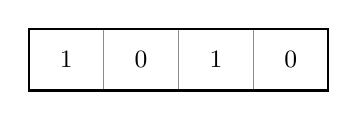
\begin{tikzpicture} \draw[black!45, fill=white] (0.000,0.000) rectangle (0.950,-0.779); \node[font=\small, text=black] at (0.475,-0.389) {$1$}; \draw[black!45, fill=white] (0.950,0.000) rectangle (1.900,-0.779); \node[font=\small, text=black] at (1.425,-0.389) {$0$}; \draw[black!45, fill=white] (1.900,0.000) rectangle (2.850,-0.779); \node[font=\small, text=black] at (2.375,-0.389) {$1$}; \draw[black!45, fill=white] (2.850,0.000) rectangle (3.800,-0.779); \node[font=\small, text=black] at (3.325,-0.389) {$0$}; \draw[line width=0.9pt] (0.000,0.000) rectangle (3.800,-0.779); \end{tikzpicture}}}$ & \tok{waste}\\[3pt]
square each entry & $\vcenter{\hbox{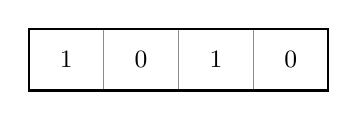
\begin{tikzpicture} \draw[black!45, fill=white] (0.000,0.000) rectangle (0.950,-0.779); \node[font=\small, text=black] at (0.475,-0.389) {$1$}; \draw[black!45, fill=white] (0.950,0.000) rectangle (1.900,-0.779); \node[font=\small, text=black] at (1.425,-0.389) {$0$}; \draw[black!45, fill=white] (1.900,0.000) rectangle (2.850,-0.779); \node[font=\small, text=black] at (2.375,-0.389) {$1$}; \draw[black!45, fill=white] (2.850,0.000) rectangle (3.800,-0.779); \node[font=\small, text=black] at (3.325,-0.389) {$0$}; \draw[line width=0.9pt] (0.000,0.000) rectangle (3.800,-0.779); \end{tikzpicture}}}$ & average of these $= 0.500$\\[3pt]
$\bm{x}/\RMS(\bm{x})$ & $\vcenter{\hbox{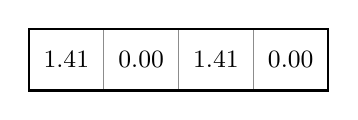
\begin{tikzpicture} \draw[black!45, fill=white] (0.000,0.000) rectangle (0.950,-0.779); \node[font=\small, text=black] at (0.475,-0.389) {$1.41$}; \draw[black!45, fill=white] (0.950,0.000) rectangle (1.900,-0.779); \node[font=\small, text=black] at (1.425,-0.389) {$0.00$}; \draw[black!45, fill=white] (1.900,0.000) rectangle (2.850,-0.779); \node[font=\small, text=black] at (2.375,-0.389) {$1.41$}; \draw[black!45, fill=white] (2.850,0.000) rectangle (3.800,-0.779); \node[font=\small, text=black] at (3.325,-0.389) {$0.00$}; \draw[line width=0.9pt] (0.000,0.000) rectangle (3.800,-0.779); \end{tikzpicture}}}$ & $\RMS = \sqrt{0.500} = 0.707$; divide every entry\\[3pt]
times gain $\bm{g}$ & $\vcenter{\hbox{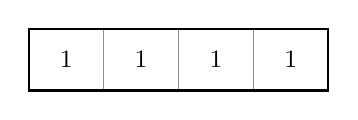
\begin{tikzpicture} \draw[black!45, fill=white] (0.000,0.000) rectangle (0.950,-0.779); \node[font=\small, text=black] at (0.475,-0.389) {$1$}; \draw[black!45, fill=white] (0.950,0.000) rectangle (1.900,-0.779); \node[font=\small, text=black] at (1.425,-0.389) {$1$}; \draw[black!45, fill=white] (1.900,0.000) rectangle (2.850,-0.779); \node[font=\small, text=black] at (2.375,-0.389) {$1$}; \draw[black!45, fill=white] (2.850,0.000) rectangle (3.800,-0.779); \node[font=\small, text=black] at (3.325,-0.389) {$1$}; \draw[line width=0.9pt] (0.000,0.000) rectangle (3.800,-0.779); \end{tikzpicture}}}$ & the toy's gain: all 1 (learned in real models)\\[3pt]
output & $\vcenter{\hbox{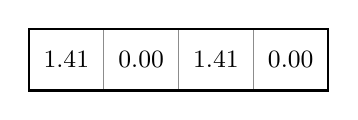
\begin{tikzpicture} \draw[black!45, fill=white] (0.000,0.000) rectangle (0.950,-0.779); \node[font=\small, text=black] at (0.475,-0.389) {$1.41$}; \draw[black!45, fill=white] (0.950,0.000) rectangle (1.900,-0.779); \node[font=\small, text=black] at (1.425,-0.389) {$0.00$}; \draw[black!45, fill=white] (1.900,0.000) rectangle (2.850,-0.779); \node[font=\small, text=black] at (2.375,-0.389) {$1.41$}; \draw[black!45, fill=white] (2.850,0.000) rectangle (3.800,-0.779); \node[font=\small, text=black] at (3.325,-0.389) {$0.00$}; \draw[line width=0.9pt] (0.000,0.000) rectangle (3.800,-0.779); \end{tikzpicture}}}$ & length $= 2.000 = \sqrt{d}$\\[3pt]
\end{tabular}

\captionof{figure}{RMSNorm on \tok{waste}, one step per line. Read down: square, average, square root, divide, multiply
by the gain. The direction never changes; only the length does.}
\end{minipage}\par\medskip

\textbf{LayerNorm} (Ba, Kiros and Hinton, 2016) does one more thing first. It subtracts the average of the
entries, then divides by their spread:
\[
\operatorname{LayerNorm}(\bm{x}) = \frac{\bm{x}-\mu}{\sigma}, \qquad \mu=\tfrac1d\textstyle\sum_i x_i,\quad
\sigma=\sqrt{\tfrac1d\textstyle\sum_i (x_i-\mu)^2}.
\]
For \tok{waste}: $\mu=\nSixMeanWaste$, and the result is $\nSixLnWaste$, also of length 2:

\par\medskip\noindent\begin{minipage}{\linewidth}\centering
% AUTO-GENERATED by code/ch6_figs.py
\begin{tabular}{@{}r@{\hspace{8pt}}c@{\hspace{8pt}}l@{}}
input $\bm{x}$ & $\vcenter{\hbox{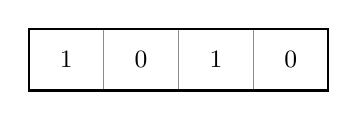
\begin{tikzpicture} \draw[black!45, fill=white] (0.000,0.000) rectangle (0.950,-0.779); \node[font=\small, text=black] at (0.475,-0.389) {$1$}; \draw[black!45, fill=white] (0.950,0.000) rectangle (1.900,-0.779); \node[font=\small, text=black] at (1.425,-0.389) {$0$}; \draw[black!45, fill=white] (1.900,0.000) rectangle (2.850,-0.779); \node[font=\small, text=black] at (2.375,-0.389) {$1$}; \draw[black!45, fill=white] (2.850,0.000) rectangle (3.800,-0.779); \node[font=\small, text=black] at (3.325,-0.389) {$0$}; \draw[line width=0.9pt] (0.000,0.000) rectangle (3.800,-0.779); \end{tikzpicture}}}$ & \tok{waste}\\[3pt]
minus the mean $\mu$ & $\vcenter{\hbox{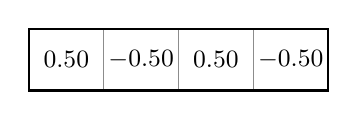
\begin{tikzpicture} \draw[black!45, fill=white] (0.000,0.000) rectangle (0.950,-0.779); \node[font=\small, text=black] at (0.475,-0.389) {$0.50$}; \draw[black!45, fill=white] (0.950,0.000) rectangle (1.900,-0.779); \node[font=\small, text=black] at (1.425,-0.389) {$-0.50$}; \draw[black!45, fill=white] (1.900,0.000) rectangle (2.850,-0.779); \node[font=\small, text=black] at (2.375,-0.389) {$0.50$}; \draw[black!45, fill=white] (2.850,0.000) rectangle (3.800,-0.779); \node[font=\small, text=black] at (3.325,-0.389) {$-0.50$}; \draw[line width=0.9pt] (0.000,0.000) rectangle (3.800,-0.779); \end{tikzpicture}}}$ & $\mu = 0.500$, subtracted from every entry\\[3pt]
divide by $\sigma$ & $\vcenter{\hbox{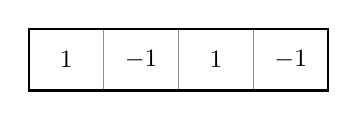
\begin{tikzpicture} \draw[black!45, fill=white] (0.000,0.000) rectangle (0.950,-0.779); \node[font=\small, text=black] at (0.475,-0.389) {$1$}; \draw[black!45, fill=white] (0.950,0.000) rectangle (1.900,-0.779); \node[font=\small, text=black] at (1.425,-0.389) {$-1$}; \draw[black!45, fill=white] (1.900,0.000) rectangle (2.850,-0.779); \node[font=\small, text=black] at (2.375,-0.389) {$1$}; \draw[black!45, fill=white] (2.850,0.000) rectangle (3.800,-0.779); \node[font=\small, text=black] at (3.325,-0.389) {$-1$}; \draw[line width=0.9pt] (0.000,0.000) rectangle (3.800,-0.779); \end{tikzpicture}}}$ & $\sigma = 0.500$, the spread of the line above\\[3pt]
times gain $\bm{g}$ & $\vcenter{\hbox{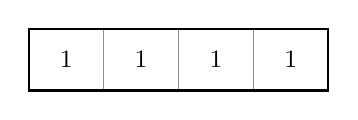
\begin{tikzpicture} \draw[black!45, fill=white] (0.000,0.000) rectangle (0.950,-0.779); \node[font=\small, text=black] at (0.475,-0.389) {$1$}; \draw[black!45, fill=white] (0.950,0.000) rectangle (1.900,-0.779); \node[font=\small, text=black] at (1.425,-0.389) {$1$}; \draw[black!45, fill=white] (1.900,0.000) rectangle (2.850,-0.779); \node[font=\small, text=black] at (2.375,-0.389) {$1$}; \draw[black!45, fill=white] (2.850,0.000) rectangle (3.800,-0.779); \node[font=\small, text=black] at (3.325,-0.389) {$1$}; \draw[line width=0.9pt] (0.000,0.000) rectangle (3.800,-0.779); \end{tikzpicture}}}$ & all 1 in the toy\\[3pt]
output & $\vcenter{\hbox{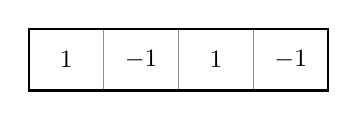
\begin{tikzpicture} \draw[black!45, fill=white] (0.000,0.000) rectangle (0.950,-0.779); \node[font=\small, text=black] at (0.475,-0.389) {$1$}; \draw[black!45, fill=white] (0.950,0.000) rectangle (1.900,-0.779); \node[font=\small, text=black] at (1.425,-0.389) {$-1$}; \draw[black!45, fill=white] (1.900,0.000) rectangle (2.850,-0.779); \node[font=\small, text=black] at (2.375,-0.389) {$1$}; \draw[black!45, fill=white] (2.850,0.000) rectangle (3.800,-0.779); \node[font=\small, text=black] at (3.325,-0.389) {$-1$}; \draw[line width=0.9pt] (0.000,0.000) rectangle (3.800,-0.779); \end{tikzpicture}}}$ & entries add to 0; length $= 2.000$\\[3pt]
\end{tabular}

\captionof{figure}{LayerNorm on \tok{waste}. The extra step is the second line: the average is taken away from every
entry, so the output's entries always add to zero.}
\end{minipage}\par\medskip

\noindent Geometrically,
subtracting the average moves the arrow onto the flat slice of space where the entries add to zero; dividing then
puts it on the sphere. So LayerNorm ignores any amount added equally to every entry: $\nSixShift$ gives the same
$\nSixLnShift$, while RMSNorm turns it into $\nSixRmsShift$.

A whole sentence goes through the norm at once, as a $T\times d$ matrix, and every row is resized with its own
RMS. Look at the middle column: \tok{waste} and \tok{time} share an RMS, \tok{of} has a smaller one, and each row
is divided only by its own number.

\par\medskip\noindent\begin{minipage}{\linewidth}\centering
% AUTO-GENERATED by code/ch6_figs.py
$\vcenter{\hbox{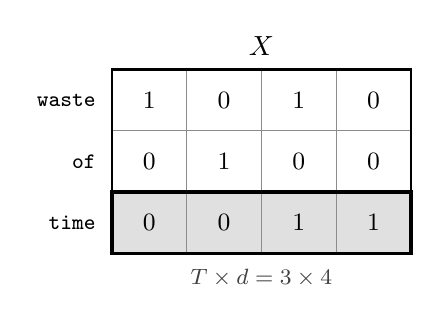
\begin{tikzpicture} \draw[black!45, fill=white] (0.000,0.000) rectangle (0.950,-0.779); \node[font=\small, text=black] at (0.475,-0.389) {$1$}; \draw[black!45, fill=white] (0.950,0.000) rectangle (1.900,-0.779); \node[font=\small, text=black] at (1.425,-0.389) {$0$}; \draw[black!45, fill=white] (1.900,0.000) rectangle (2.850,-0.779); \node[font=\small, text=black] at (2.375,-0.389) {$1$}; \draw[black!45, fill=white] (2.850,0.000) rectangle (3.800,-0.779); \node[font=\small, text=black] at (3.325,-0.389) {$0$}; \draw[black!45, fill=white] (0.000,-0.779) rectangle (0.950,-1.558); \node[font=\small, text=black] at (0.475,-1.168) {$0$}; \draw[black!45, fill=white] (0.950,-0.779) rectangle (1.900,-1.558); \node[font=\small, text=black] at (1.425,-1.168) {$1$}; \draw[black!45, fill=white] (1.900,-0.779) rectangle (2.850,-1.558); \node[font=\small, text=black] at (2.375,-1.168) {$0$}; \draw[black!45, fill=white] (2.850,-0.779) rectangle (3.800,-1.558); \node[font=\small, text=black] at (3.325,-1.168) {$0$}; \draw[black!45, fill=black!12] (0.000,-1.558) rectangle (0.950,-2.337); \node[font=\small, text=black] at (0.475,-1.947) {$0$}; \draw[black!45, fill=black!12] (0.950,-1.558) rectangle (1.900,-2.337); \node[font=\small, text=black] at (1.425,-1.947) {$0$}; \draw[black!45, fill=black!12] (1.900,-1.558) rectangle (2.850,-2.337); \node[font=\small, text=black] at (2.375,-1.947) {$1$}; \draw[black!45, fill=black!12] (2.850,-1.558) rectangle (3.800,-2.337); \node[font=\small, text=black] at (3.325,-1.947) {$1$}; \draw[line width=1.4pt] (0.000,-1.558) rectangle (3.800,-2.337); \draw[line width=0.9pt] (0.000,0.000) rectangle (3.800,-2.337); \node[anchor=east, font=\footnotesize\ttfamily] at (-0.080,-0.389) {waste}; \node[anchor=east, font=\footnotesize\ttfamily] at (-0.080,-1.168) {of}; \node[anchor=east, font=\footnotesize\ttfamily] at (-0.080,-1.947) {time}; \node[anchor=south, font=\normalsize] at (1.900,0.050) {$X$}; \node[anchor=north, font=\footnotesize, text=black!75] at (1.900,-2.417) {$T\times d=3\times4$}; \end{tikzpicture}}}$\ \ {\Large$\div$}\ \ $\vcenter{\hbox{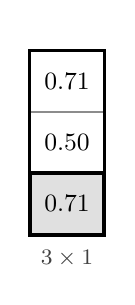
\begin{tikzpicture} \draw[black!45, fill=white] (0.000,0.000) rectangle (0.950,-0.779); \node[font=\small, text=black] at (0.475,-0.389) {$0.71$}; \draw[black!45, fill=white] (0.000,-0.779) rectangle (0.950,-1.558); \node[font=\small, text=black] at (0.475,-1.168) {$0.50$}; \draw[black!45, fill=black!12] (0.000,-1.558) rectangle (0.950,-2.337); \node[font=\small, text=black] at (0.475,-1.947) {$0.71$}; \draw[line width=1.4pt] (0.000,-1.558) rectangle (0.950,-2.337); \draw[line width=0.9pt] (0.000,0.000) rectangle (0.950,-2.337); \node[anchor=south, font=\normalsize] at (0.475,0.050) {$\RMS$}; \node[anchor=north, font=\footnotesize, text=black!75] at (0.475,-2.417) {$3\times1$}; \end{tikzpicture}}}$\ \ {\Large$=$}\ \ $\vcenter{\hbox{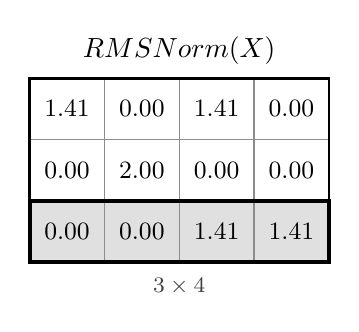
\begin{tikzpicture} \draw[black!45, fill=white] (0.000,0.000) rectangle (0.950,-0.779); \node[font=\small, text=black] at (0.475,-0.389) {$1.41$}; \draw[black!45, fill=white] (0.950,0.000) rectangle (1.900,-0.779); \node[font=\small, text=black] at (1.425,-0.389) {$0.00$}; \draw[black!45, fill=white] (1.900,0.000) rectangle (2.850,-0.779); \node[font=\small, text=black] at (2.375,-0.389) {$1.41$}; \draw[black!45, fill=white] (2.850,0.000) rectangle (3.800,-0.779); \node[font=\small, text=black] at (3.325,-0.389) {$0.00$}; \draw[black!45, fill=white] (0.000,-0.779) rectangle (0.950,-1.558); \node[font=\small, text=black] at (0.475,-1.168) {$0.00$}; \draw[black!45, fill=white] (0.950,-0.779) rectangle (1.900,-1.558); \node[font=\small, text=black] at (1.425,-1.168) {$2.00$}; \draw[black!45, fill=white] (1.900,-0.779) rectangle (2.850,-1.558); \node[font=\small, text=black] at (2.375,-1.168) {$0.00$}; \draw[black!45, fill=white] (2.850,-0.779) rectangle (3.800,-1.558); \node[font=\small, text=black] at (3.325,-1.168) {$0.00$}; \draw[black!45, fill=black!12] (0.000,-1.558) rectangle (0.950,-2.337); \node[font=\small, text=black] at (0.475,-1.947) {$0.00$}; \draw[black!45, fill=black!12] (0.950,-1.558) rectangle (1.900,-2.337); \node[font=\small, text=black] at (1.425,-1.947) {$0.00$}; \draw[black!45, fill=black!12] (1.900,-1.558) rectangle (2.850,-2.337); \node[font=\small, text=black] at (2.375,-1.947) {$1.41$}; \draw[black!45, fill=black!12] (2.850,-1.558) rectangle (3.800,-2.337); \node[font=\small, text=black] at (3.325,-1.947) {$1.41$}; \draw[line width=1.4pt] (0.000,-1.558) rectangle (3.800,-2.337); \draw[line width=0.9pt] (0.000,0.000) rectangle (3.800,-2.337); \node[anchor=south, font=\normalsize] at (1.900,0.050) {$\operatorname{RMSNorm}(X)$}; \node[anchor=north, font=\footnotesize, text=black!75] at (1.900,-2.417) {$3\times4$}; \end{tikzpicture}}}$

\captionof{figure}{RMSNorm on the sentence matrix. The highlighted row, \tok{time}, is divided by its own RMS,
\nSixRmsValTime; no row borrows another row's number. The LayerNorm of each row follows the same rule with
mean and spread.}
\end{minipage}\par\medskip

Real models then multiply each coordinate by a learned \emph{gain} (and LayerNorm adds a learned shift), so the
model can choose the size it wants per coordinate. In our toy every gain is 1.

\begin{breaks}
Resizing photos treats each photo on its own, and so does the norm: it rescales one token's arrow using only that
token's numbers. It does not make tokens equal to each other in content, and it does not compare them.
\end{breaks}

The same holds for a batch. Two customer replies stacked as a $B\times T\times d$ block go in; the same block
shape comes out, and every one of the six rows has been resized on its own:

\par\medskip\noindent\begin{minipage}{\linewidth}\centering
% AUTO-GENERATED by code/ch6_figs.py
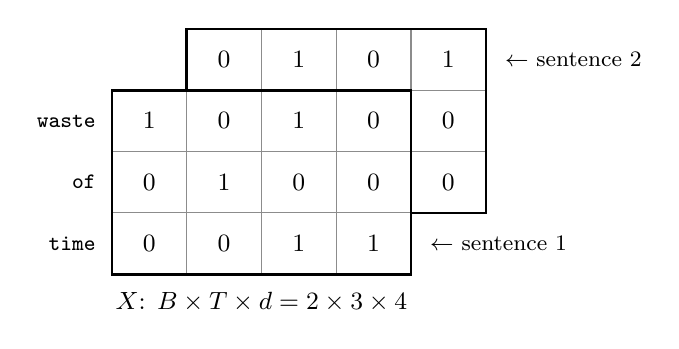
\begin{tikzpicture}
\fill[white] (0.950,0.779) rectangle (4.750,-1.558);
\draw[black!45, fill=white] (0.950,0.779) rectangle (1.900,0.000);
\node[font=\small, text=black] at (1.425,0.389) {$0$};
\draw[black!45, fill=white] (1.900,0.779) rectangle (2.850,0.000);
\node[font=\small, text=black] at (2.375,0.389) {$1$};
\draw[black!45, fill=white] (2.850,0.779) rectangle (3.800,0.000);
\node[font=\small, text=black] at (3.325,0.389) {$0$};
\draw[black!45, fill=white] (3.800,0.779) rectangle (4.750,0.000);
\node[font=\small, text=black] at (4.275,0.389) {$1$};
\draw[black!45, fill=white] (0.950,0.000) rectangle (1.900,-0.779);
\node[font=\small, text=black] at (1.425,-0.389) {$1$};
\draw[black!45, fill=white] (1.900,0.000) rectangle (2.850,-0.779);
\node[font=\small, text=black] at (2.375,-0.389) {$0$};
\draw[black!45, fill=white] (2.850,0.000) rectangle (3.800,-0.779);
\node[font=\small, text=black] at (3.325,-0.389) {$0$};
\draw[black!45, fill=white] (3.800,0.000) rectangle (4.750,-0.779);
\node[font=\small, text=black] at (4.275,-0.389) {$0$};
\draw[black!45, fill=white] (0.950,-0.779) rectangle (1.900,-1.558);
\node[font=\small, text=black] at (1.425,-1.168) {$0$};
\draw[black!45, fill=white] (1.900,-0.779) rectangle (2.850,-1.558);
\node[font=\small, text=black] at (2.375,-1.168) {$0$};
\draw[black!45, fill=white] (2.850,-0.779) rectangle (3.800,-1.558);
\node[font=\small, text=black] at (3.325,-1.168) {$1$};
\draw[black!45, fill=white] (3.800,-0.779) rectangle (4.750,-1.558);
\node[font=\small, text=black] at (4.275,-1.168) {$0$};
\draw[line width=0.9pt] (0.950,0.779) rectangle (4.750,-1.558);
\node[anchor=west, font=\footnotesize] at (4.870,0.389) {$\leftarrow$ sentence 2};
\fill[white] (0.000,0.000) rectangle (3.800,-2.337);
\draw[black!45, fill=white] (0.000,0.000) rectangle (0.950,-0.779);
\node[font=\small, text=black] at (0.475,-0.389) {$1$};
\draw[black!45, fill=white] (0.950,0.000) rectangle (1.900,-0.779);
\node[font=\small, text=black] at (1.425,-0.389) {$0$};
\draw[black!45, fill=white] (1.900,0.000) rectangle (2.850,-0.779);
\node[font=\small, text=black] at (2.375,-0.389) {$1$};
\draw[black!45, fill=white] (2.850,0.000) rectangle (3.800,-0.779);
\node[font=\small, text=black] at (3.325,-0.389) {$0$};
\draw[black!45, fill=white] (0.000,-0.779) rectangle (0.950,-1.558);
\node[font=\small, text=black] at (0.475,-1.168) {$0$};
\draw[black!45, fill=white] (0.950,-0.779) rectangle (1.900,-1.558);
\node[font=\small, text=black] at (1.425,-1.168) {$1$};
\draw[black!45, fill=white] (1.900,-0.779) rectangle (2.850,-1.558);
\node[font=\small, text=black] at (2.375,-1.168) {$0$};
\draw[black!45, fill=white] (2.850,-0.779) rectangle (3.800,-1.558);
\node[font=\small, text=black] at (3.325,-1.168) {$0$};
\draw[black!45, fill=white] (0.000,-1.558) rectangle (0.950,-2.337);
\node[font=\small, text=black] at (0.475,-1.947) {$0$};
\draw[black!45, fill=white] (0.950,-1.558) rectangle (1.900,-2.337);
\node[font=\small, text=black] at (1.425,-1.947) {$0$};
\draw[black!45, fill=white] (1.900,-1.558) rectangle (2.850,-2.337);
\node[font=\small, text=black] at (2.375,-1.947) {$1$};
\draw[black!45, fill=white] (2.850,-1.558) rectangle (3.800,-2.337);
\node[font=\small, text=black] at (3.325,-1.947) {$1$};
\draw[line width=0.9pt] (0.000,0.000) rectangle (3.800,-2.337);
\node[anchor=east, font=\footnotesize\ttfamily] at (-0.080,-0.389) {waste};
\node[anchor=east, font=\footnotesize\ttfamily] at (-0.080,-1.168) {of};
\node[anchor=east, font=\footnotesize\ttfamily] at (-0.080,-1.947) {time};
\node[anchor=west, font=\footnotesize] at (3.920,-1.947) {$\leftarrow$ sentence 1};
\node[anchor=north, font=\small] at (1.900,-2.437) {$X$: $B\times T\times d = 2\times3\times4$};
\end{tikzpicture}\\[6pt]{\Large$\Downarrow$}\ \small each of the six rows divided by its own RMS\\[6pt]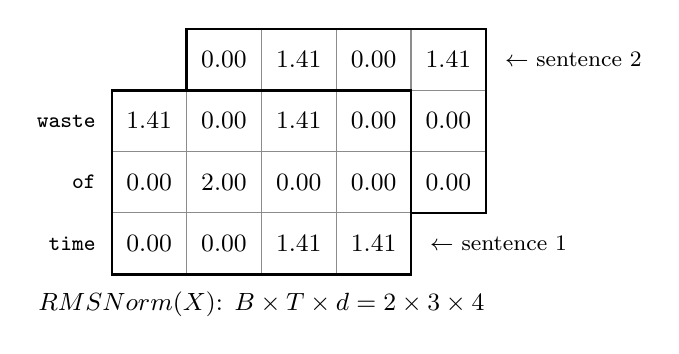
\begin{tikzpicture}
\fill[white] (0.950,0.779) rectangle (4.750,-1.558);
\draw[black!45, fill=white] (0.950,0.779) rectangle (1.900,0.000);
\node[font=\small, text=black] at (1.425,0.389) {$0.00$};
\draw[black!45, fill=white] (1.900,0.779) rectangle (2.850,0.000);
\node[font=\small, text=black] at (2.375,0.389) {$1.41$};
\draw[black!45, fill=white] (2.850,0.779) rectangle (3.800,0.000);
\node[font=\small, text=black] at (3.325,0.389) {$0.00$};
\draw[black!45, fill=white] (3.800,0.779) rectangle (4.750,0.000);
\node[font=\small, text=black] at (4.275,0.389) {$1.41$};
\draw[black!45, fill=white] (0.950,0.000) rectangle (1.900,-0.779);
\node[font=\small, text=black] at (1.425,-0.389) {$2.00$};
\draw[black!45, fill=white] (1.900,0.000) rectangle (2.850,-0.779);
\node[font=\small, text=black] at (2.375,-0.389) {$0.00$};
\draw[black!45, fill=white] (2.850,0.000) rectangle (3.800,-0.779);
\node[font=\small, text=black] at (3.325,-0.389) {$0.00$};
\draw[black!45, fill=white] (3.800,0.000) rectangle (4.750,-0.779);
\node[font=\small, text=black] at (4.275,-0.389) {$0.00$};
\draw[black!45, fill=white] (0.950,-0.779) rectangle (1.900,-1.558);
\node[font=\small, text=black] at (1.425,-1.168) {$0.00$};
\draw[black!45, fill=white] (1.900,-0.779) rectangle (2.850,-1.558);
\node[font=\small, text=black] at (2.375,-1.168) {$0.00$};
\draw[black!45, fill=white] (2.850,-0.779) rectangle (3.800,-1.558);
\node[font=\small, text=black] at (3.325,-1.168) {$2.00$};
\draw[black!45, fill=white] (3.800,-0.779) rectangle (4.750,-1.558);
\node[font=\small, text=black] at (4.275,-1.168) {$0.00$};
\draw[line width=0.9pt] (0.950,0.779) rectangle (4.750,-1.558);
\node[anchor=west, font=\footnotesize] at (4.870,0.389) {$\leftarrow$ sentence 2};
\fill[white] (0.000,0.000) rectangle (3.800,-2.337);
\draw[black!45, fill=white] (0.000,0.000) rectangle (0.950,-0.779);
\node[font=\small, text=black] at (0.475,-0.389) {$1.41$};
\draw[black!45, fill=white] (0.950,0.000) rectangle (1.900,-0.779);
\node[font=\small, text=black] at (1.425,-0.389) {$0.00$};
\draw[black!45, fill=white] (1.900,0.000) rectangle (2.850,-0.779);
\node[font=\small, text=black] at (2.375,-0.389) {$1.41$};
\draw[black!45, fill=white] (2.850,0.000) rectangle (3.800,-0.779);
\node[font=\small, text=black] at (3.325,-0.389) {$0.00$};
\draw[black!45, fill=white] (0.000,-0.779) rectangle (0.950,-1.558);
\node[font=\small, text=black] at (0.475,-1.168) {$0.00$};
\draw[black!45, fill=white] (0.950,-0.779) rectangle (1.900,-1.558);
\node[font=\small, text=black] at (1.425,-1.168) {$2.00$};
\draw[black!45, fill=white] (1.900,-0.779) rectangle (2.850,-1.558);
\node[font=\small, text=black] at (2.375,-1.168) {$0.00$};
\draw[black!45, fill=white] (2.850,-0.779) rectangle (3.800,-1.558);
\node[font=\small, text=black] at (3.325,-1.168) {$0.00$};
\draw[black!45, fill=white] (0.000,-1.558) rectangle (0.950,-2.337);
\node[font=\small, text=black] at (0.475,-1.947) {$0.00$};
\draw[black!45, fill=white] (0.950,-1.558) rectangle (1.900,-2.337);
\node[font=\small, text=black] at (1.425,-1.947) {$0.00$};
\draw[black!45, fill=white] (1.900,-1.558) rectangle (2.850,-2.337);
\node[font=\small, text=black] at (2.375,-1.947) {$1.41$};
\draw[black!45, fill=white] (2.850,-1.558) rectangle (3.800,-2.337);
\node[font=\small, text=black] at (3.325,-1.947) {$1.41$};
\draw[line width=0.9pt] (0.000,0.000) rectangle (3.800,-2.337);
\node[anchor=east, font=\footnotesize\ttfamily] at (-0.080,-0.389) {waste};
\node[anchor=east, font=\footnotesize\ttfamily] at (-0.080,-1.168) {of};
\node[anchor=east, font=\footnotesize\ttfamily] at (-0.080,-1.947) {time};
\node[anchor=west, font=\footnotesize] at (3.920,-1.947) {$\leftarrow$ sentence 1};
\node[anchor=north, font=\small] at (1.900,-2.437) {$\operatorname{RMSNorm}(X)$: $B\times T\times d = 2\times3\times4$};
\end{tikzpicture}

\captionof{figure}{RMSNorm on a batch of $B=2$ sentences. Shape in, shape out: $2\times3\times4$. No number moves between
rows, and none moves between sentences.}
\end{minipage}\par\medskip

\Why The norm removes the one thing depth messes up, the size, and keeps the thing the model needs, the
direction. Chapter 3 showed that a dot product has two knobs, direction and length; normalisation fixes the
length knob of the input so that what a block computes depends on direction alone. RMSNorm skips the centring
step, which costs a little computation and, in Zhang and Sennrich's experiments, lost nothing; Llama and Qwen use
it.

\begin{wrongidea}{6.1}
\emph{Normalisation is there so that no token can beat another.} It is tempting because the word sounds like making things
fair. But the norm acts on each token alone and keeps its direction, so tokens still differ as much as before.
What it controls is the size of each arrow as it goes through many layers.
\end{wrongidea}

\begin{wrongidea}{6.2}
\emph{Normalising throws away the information in an arrow.} Only the length is removed (and, for LayerNorm, the
average entry). The direction, which is where the meaning lives, is untouched.
\end{wrongidea}

\begin{wrongidea}{6.3}
\emph{LayerNorm makes every arrow length 1.} It makes the entries' spread 1, so the length is $\sqrt d$: 2 in our
toy, about 32 for $d=1024$. ``Unit length'' is a different, related idea.
\end{wrongidea}

\begin{checkq}
What does RMSNorm do to the arrow $(2,0,2,0)$?
\begin{options}
\item It returns $\nSixRmsWaste$, the same as for $(1,0,1,0)$.
\item It returns $(1,0,1,0)$, an arrow of length 1.
\item It returns $(1,-1,1,-1)$, after removing the average.
\item It makes it equal to the RMSNorm of \tok{time}, so the two tokens can no longer be told apart.
\end{options}
\end{checkq}

\Summary{A norm rescales each token's arrow to a fixed length, $\sqrt d$, and keeps its direction.}

%---------------------------------------------------------------------
\subsection*{6.3\quad The toy block with a norm}

Where does the norm go? In modern models, in front of each layer's input, and once more before the output:
\[
\bm{h}_1 = \bm{x} + \operatorname{Attn}(\operatorname{Norm}(\bm{x})), \qquad
\bm{h}_2 = \bm{h}_1 + \operatorname{MLP}(\operatorname{Norm}(\bm{h}_1)), \qquad
\text{output reads } \operatorname{Norm}(\bm{h}_2).
\]
Notice that the norm sits on the side road into each layer, not on the residual stream itself. The stream is
still only ever added to.

\Predict With RMSNorm in front, the attention inputs have length 2 instead of about 1.4. Will the heads become
more decisive or less? Recall the length knob of Chapter 3, \S3.7.

\Sanity More decisive. \tok{waste} enters attention as $\nSixAttnInWaste$. Head 1's shares for \tok{time} move
from $\nSixAoneNone$ without the norm to $\nSixAoneRms$ with it; head 2's from $\nSixAtwoNone$ to
$\nSixAtwoRms$. Longer arrows, sharper softmax.

The three MLP neurons still fire on their own rows only, now with strengths $\nSixActRmsDiag$ instead of
$\nSixActNoneDiag$, and the toy still predicts \nSixPredRms\ at the three positions. Chapter 7 starts from exactly
this block.

What if we swap in LayerNorm, keeping every weight the same? The predictions become \nSixPredLayer: the first
position now prefers \tok{\nSixLnTopWaste} (score \nSixLnTopWasteLogit) over \tok{of} (\nSixLnOfLogit). Our
hand-chosen weights were checked with RMSNorm, and LayerNorm sends the arrows to different places. A trained
model learns its weights together with its norm; swapping the norm afterwards breaks it in the same way.

\Summary{With pre-norm the toy keeps its three correct guesses and its heads become sharper, because every input
now has the same length.}

%---------------------------------------------------------------------
\subsection*{6.4\quad Before or after? A measured choice}

There are two places to put the norm.
\begin{itemize}
\item \textbf{Post-norm} (the original transformer, Vaswani and colleagues, 2017): add, then normalise the
stream itself: $\bm{x}\leftarrow\operatorname{Norm}(\bm{x}+F(\bm{x}))$.
\item \textbf{Pre-norm} (GPT-2 and most models since): normalise the copy that goes into the layer, add the
result to the untouched stream: $\bm{x}\leftarrow\bm{x}+F(\operatorname{Norm}(\bm{x}))$.
\end{itemize}

\Predict Both keep sizes under control. Which one lets the top of a 48-layer stack still see the token that came
in at the bottom?

\Picture Post-norm is a notebook that gets photocopied at a fixed size after every note is added. Each copy
shrinks the older writing to make room, so after many copies the first page is a speck. Pre-norm gives each desk a
resized copy to read, but every desk writes on the original notebook, which keeps all the old writing at full
size.

\Exactly We measured both on the same 48 untrained blocks. ``Agreement with the input'' is the cosine of the angle
between each position's arrow at layer $L$ and its arrow at the start (1 means same direction, 0 means
unrelated). ``Knows its token'' is the test from Chapter 5.

\begin{center}
\small
\begin{tabular}{@{}l r r r r r@{}}
\toprule
layers $L$ & 1 & 6 & 12 & 24 & 48\\
\midrule
size (RMS), post-norm & \nSixRmsPostOne & \nSixRmsPostSix & \nSixRmsPostTwelve & \nSixRmsPostTwentyFour & \nSixRmsPostFortyEight\\
size (RMS), pre-norm & \nSixRmsPreOne & \nSixRmsPreSix & \nSixRmsPreTwelve & \nSixRmsPreTwentyFour & \nSixRmsPreFortyEight\\
agreement with input, post-norm & \nSixCosPostOne & \nSixCosPostSix & \nSixCosPostTwelve & \nSixCosPostTwentyFour & \nSixCosPostFortyEight\\
agreement with input, pre-norm & \nSixCosPreOne & \nSixCosPreSix & \nSixCosPreTwelve & \nSixCosPreTwentyFour & \nSixCosPreFortyEight\\
knows its token, post-norm (\%) & \nSixIdPostOne & \nSixIdPostSix & \nSixIdPostTwelve & \nSixIdPostTwentyFour & \nSixIdPostFortyEight\\
knows its token, pre-norm (\%) & \nSixIdPreOne & \nSixIdPreSix & \nSixIdPreTwelve & \nSixIdPreTwentyFour & \nSixIdPreFortyEight\\
\bottomrule
\end{tabular}
\end{center}

\begin{figure}[h]
\centering
\begin{tikzpicture}
\begin{axis}[name=left, width=7.8cm, height=6cm, ymode=log, ymin=1e-3, xlabel={layers $L$}, ylabel={size of stream (RMS)},
  xmin=0, xmax=48, axis lines*=left, tick label style={font=\footnotesize}, label style={font=\small}]
\addplot[very thick, black] table[x=L, y=noneres] {data_ch6/depth.dat} node[pos=0.55, above left, font=\footnotesize] {no norm};
\addplot[very thick, black!75, dashed] table[x=L, y=pre] {data_ch6/depth.dat} node[pos=0.9, above, font=\footnotesize] {pre-norm};
\addplot[very thick, black!60, dotted] table[x=L, y=post] {data_ch6/depth.dat} node[pos=0.5, below=2pt, font=\footnotesize] {post-norm};
\end{axis}
\begin{axis}[at={(left.east)}, anchor=west, xshift=1.5cm, width=7.8cm, height=6cm, xlabel={layers $L$},
  ylabel={agreement with input}, xmin=0, xmax=48, ymin=-0.05, ymax=1.05, axis lines*=left,
  tick label style={font=\footnotesize}, label style={font=\small}]
\addplot[very thick, black!75, dashed] table[x=L, y=precos] {data_ch6/depth.dat} node[pos=0.5, above right, font=\footnotesize] {pre-norm};
\addplot[very thick, black!60, dotted] table[x=L, y=postcos] {data_ch6/depth.dat} node[pos=0.25, above right, font=\footnotesize] {post-norm};
\end{axis}
\end{tikzpicture}
\caption{Forty-eight untrained blocks, fixed seed. Left: without a norm the size explodes; post-norm pins it at 1;
pre-norm lets it grow slowly. Right: post-norm loses the input within a few layers; pre-norm keeps it visible
much longer.}
\end{figure}

Two readings. First, post-norm holds the size at exactly 1 (with RMSNorm, the stream's RMS is 1 by construction),
but the input's direction is gone by about 6 layers: each add-and-normalise shrinks the old content. If every
update were as large as the stream and unrelated to it, one step would keep $1/\sqrt2\approx\nSixHalfShare$ of the
old content, and six steps would keep $\nSixHalfPowSix$. Second, pre-norm lets the size grow, but slowly: from 12
to 48 layers it grows by a factor of \nSixPreRatio, close to $\sqrt{48/12}=\nSixSqrtFour$, the coin-toss growth of
Chapter 3. The input stays readable much longer because the stream itself is never rescaled.

\begin{breaks}
Our measurement looks only at the forward pass of untrained blocks. The deeper reason for pre-norm is about
learning: Xiong and colleagues (2020) showed that with post-norm the learning signals reaching the bottom layers
are badly sized at the start of training, which is why the original transformer needed a slow ``warm-up'' of the
learning rate. Appendix A gives that argument with derivatives.
\end{breaks}

\Why Pre-norm keeps a clean, untouched path from bottom to top (the residual stream) and puts the size control
only where each layer reads. Information from the bottom reaches the top without being shrunk at every step, and,
as Xiong and colleagues showed, so does the learning signal on its way down. That is why GPT-2, Llama and Qwen
all use it, plus one final norm before the output, since the stream itself is never normalised.

\begin{wrongidea}{6.5}
\emph{Whether the norm sits before or after a layer is a detail.} Both versions compute the same kinds of
things, so the placement looks cosmetic. The table shows a difference you can measure in the first few layers,
and it decides whether a deep model can be trained without special care.
\end{wrongidea}

\begin{checkq}
In a post-norm stack, why does the bottom token's direction fade even though the size stays at exactly 1?
\begin{options}
\item Because the norm throws away the direction.
\item Because each add-and-normalise step shrinks the old content to make room for the new.
\item Because the attention heads ignore the token itself.
\item Because size and direction are the same thing.
\end{options}
\end{checkq}

\begin{principle}{control what each stage reads, keep the record untouched}
Pre-norm resizes the input of every layer but never edits the stream. A reliable pipeline of agents does the same:
each step validates and normalises what it reads (a schema, a typed decision such as a yes/no answer or a
score), while the raw record of what happened is kept as it was, so a later
step can always go back to it. Normalising the record itself, step after step, slowly erases where it came from.
\end{principle}

\Summary{Pre-norm resizes each layer's input and leaves the stream alone, which keeps sizes under control and keeps
the bottom of a deep stack visible at the top.}

\begin{lookingback}
(1) In Chapter 3, why did we divide attention scores by $\sqrt{d_k}$, and which design rule did that follow?
(2) In Chapter 5, what did the residual additions keep, according to the figure in \S5.5? (3) In Chapter 1,
what happened to an RNN's memory when each step multiplied it by 0.9?
\end{lookingback}

\begin{exercise}
Compute the RMSNorm and the LayerNorm of $(0,0,1,1)$ by hand, and check both lengths.
\end{exercise}
\begin{exercise}
LayerNorm gives the same output for $(1,0,1,0)$ and $(4,3,4,3)$. Give one situation where ignoring a shift
of every entry is helpful, and one where it could lose information.
\end{exercise}
\begin{exercise}
Assume each add-and-normalise step of post-norm keeps $1/\sqrt2$ of the old content. How much is left after 6 steps?
Why is the measured agreement after 6 layers larger than this?
\end{exercise}
\begin{exercise}
In our pre-norm measurement the stream's size grows roughly like the square root of the depth. Predict its size at
192 layers from the value at 48 layers.
\end{exercise}

\subsection*{Answers to Chapter 6}
\small
\textbf{Check yourself 6.1.} (a). RMSNorm ignores the overall scale: $(2,0,2,0)$ is $(1,0,1,0)$ doubled. (b) is
M6.3: the length is $\sqrt d=2$, not 1. (c) is LayerNorm, not RMSNorm. (d) is M6.1 and M6.2: \tok{time} points
elsewhere, and its direction survives the norm.

\textbf{Check yourself 6.2.} (b). Every step rescales the sum of old and new, so the old part's share shrinks
step by step. (a) is M6.2. (c) is unrelated to the norm. (d) confuses length with direction: the norm fixes one
and keeps the other.

\textbf{Looking back.} (1) Random dot products grow like $\sqrt{d_k}$; dividing keeps the size independent of the
model's width. (2) The identity of each token: most positions still knew their token after 12 layers. (3) It faded:
$0.9^{100}\approx\hFadeHundred$.

\textbf{Exercise 6.1.} $\RMS(0,0,1,1)=\nSixRmsValTime$, so RMSNorm gives $\nSixRmsTime$. LayerNorm: $\mu=\nSixMeanTime$,
giving $\nSixLnTime$. Both have length 2.

\textbf{Exercise 6.2.} Helpful: if some input adds the same offset to every entry for a reason unrelated to meaning,
ignoring it removes noise. Losing: if the overall level of the entries carries meaning, LayerNorm erases it, while
RMSNorm keeps it.

\textbf{Exercise 6.3.} $(1/\sqrt2)^6=\nSixHalfPowSix$. Real updates are smaller than the stream and not fully
unrelated to it, so each step shrinks the old content less; the measured value after 6 layers is \nSixCosPostSix.

\textbf{Exercise 6.4.} Four times the depth gives $\sqrt4=2$ times the size: about \nSixPreRmsPredict, from
\nSixRmsPreFortyEight\ at 48 layers.
\normalsize

\subsection*{What you now know}
\begin{itemize}
\item Why stacking blocks makes arrow sizes explode or fade, with measured numbers.
\item What RMSNorm and LayerNorm do to an arrow: fix its length at $\sqrt d$, keep its direction; LayerNorm also
removes the average.
\item Where the norm sits in a modern block, and what it does to our toy's attention.
\item Why pre-norm is preferred to post-norm, measured on 48 layers, and where the full argument lives (Appendix A).
\end{itemize}
